\begin{figure}[htb]
    \centering
    \caption{Correlation Between Median Rent Price (in dollars per square foot) and previous year change in MW (percentage).}
    \label{appfig:binsc_listing_mwpctchange}
    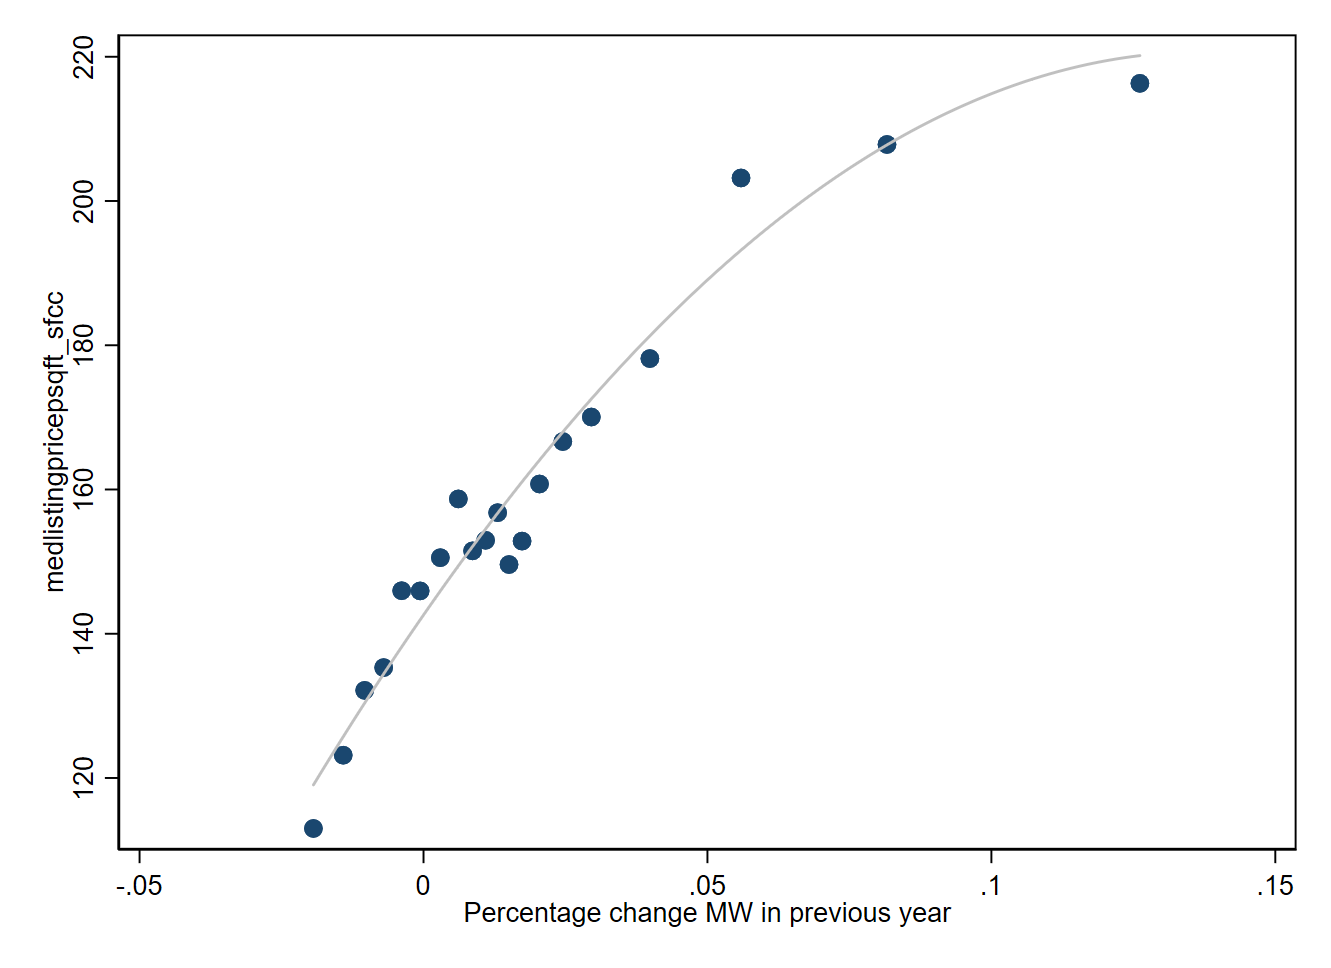
\includegraphics[width=0.75\linewidth]{draft_june20/tempfigure/binsc_medlistingpricepsqft_sfcc_pctMWch.png}
    \begin{minipage}{.95\textwidth} \footnotesize
		\vspace{2mm} 
		\textit{Notes}: The figure presents the correlation between median listing price on Zillow.com at the zipcode-year level and the percentage change in MW in the previous year. Data comes from the final sample used in the analysis (see \autoref{sec:data}, and \autoref{tab:samples_table}, column 3 for more details). Each zipcode yearly observation is obtained by averaging monthly observations, the basic time unit in this paper. The correlation is taken after controlling for year fixed effects, resident population, urban share, median income, black population share, and number of housing units.All demographic characteristics come from the 2010 Census.
	\end{minipage}
\end{figure}

\clearpage
\begin{figure}[h!] \centering
        \caption{Dynamic effects around selected minimum wage events: county-quarter level estimates}
        \label{appfig:event_study_c-q}
        \begin{subfigure}{0.5\textwidth} \centering
            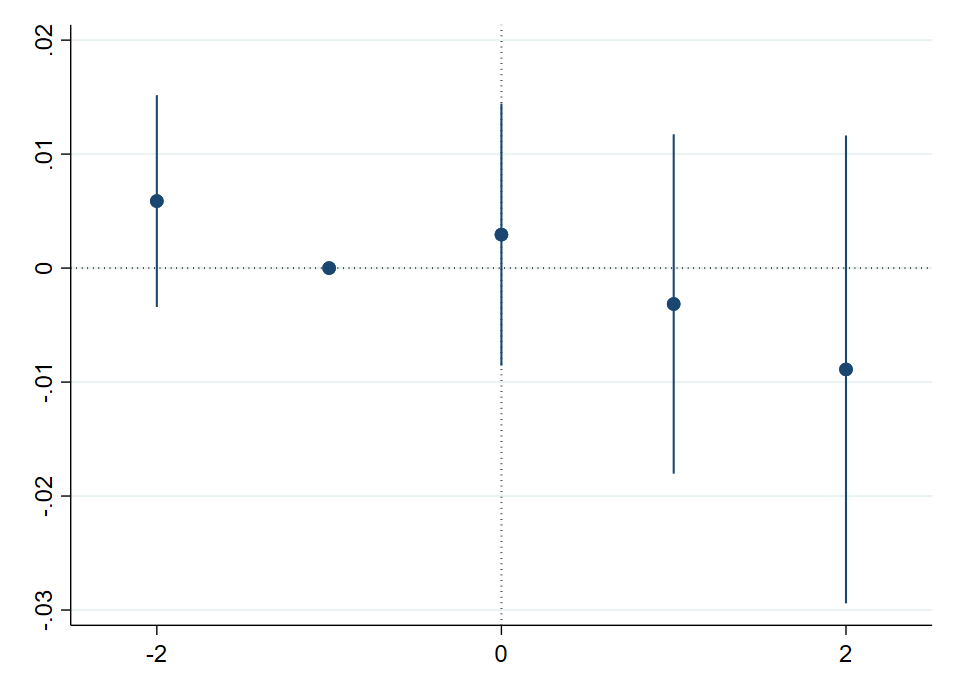
\includegraphics[width=0.95\linewidth]{analysis/event_study_county_quarter/output/last_rentpsqft_sfcc_w2.png}
            \caption{TWFE with all units and $w=2$} \label{fig:event_study_c-q_all_w2}
        \end{subfigure}%
        \begin{subfigure}{0.5\textwidth} \centering
            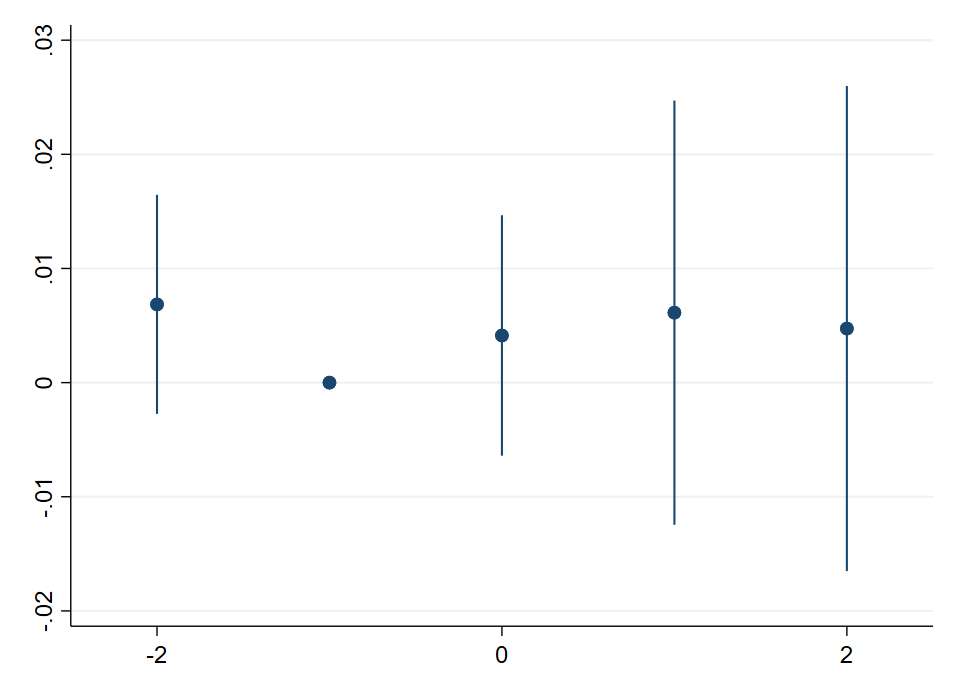
\includegraphics[width=0.95\linewidth]{analysis/event_study_county_quarter/output/last_rentpsqft_sfcc_w2_trend.png}
            \caption{\begin{tabular}{c} TWFE with all units, $w=2$ \\ and county-specific trends \end{tabular}} \label{fig:event_study_c-q_all_w2_trend}
        \end{subfigure}\\
        \begin{subfigure}{0.5\textwidth} \centering
            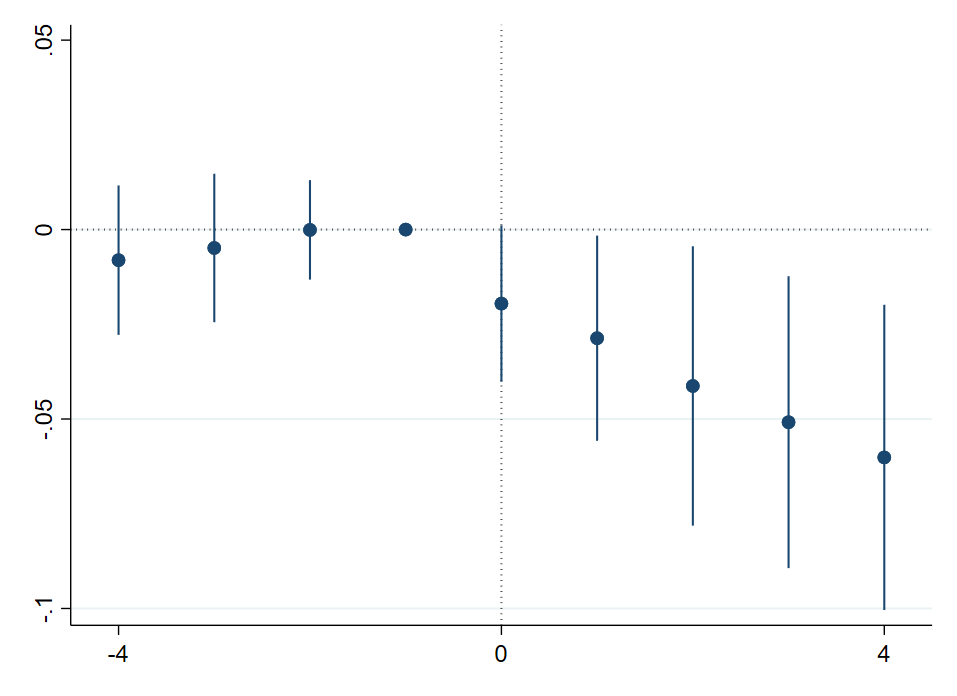
\includegraphics[width=0.95\linewidth]{analysis/event_study_county_quarter/output/last_rentpsqft_sfcc_w4.png}
            \caption{TWFE with all units and $w=4$} \label{fig:event_study_c-q_all_w4}
        \end{subfigure}%
        \begin{subfigure}{0.5\textwidth} \centering
            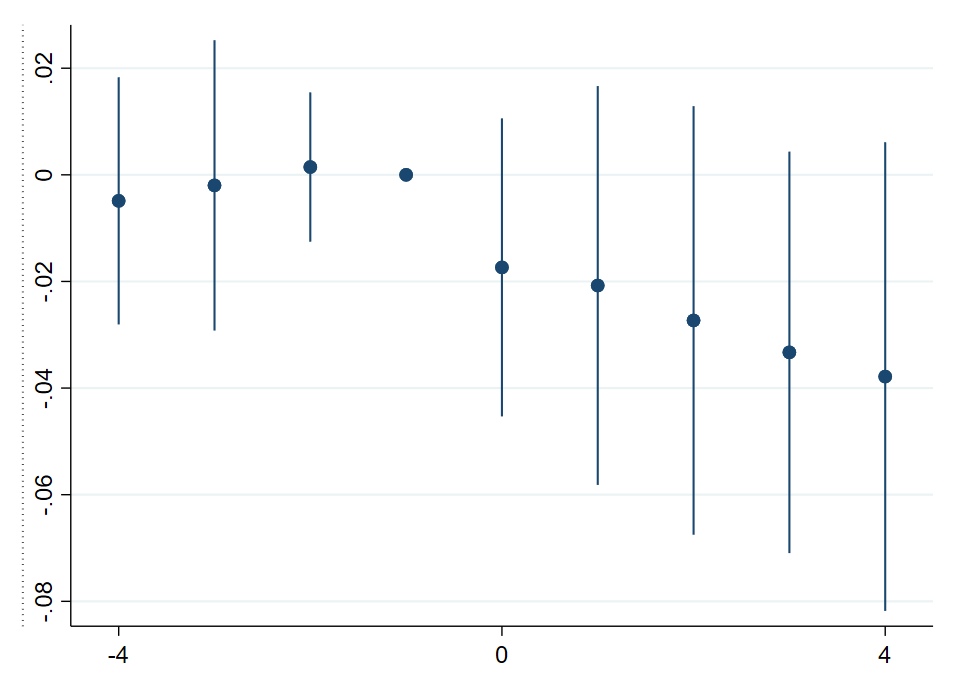
\includegraphics[width=0.95\linewidth]{analysis/event_study_county_quarter/output/last_rentpsqft_sfcc_w4_trend.png}
            \caption{\begin{tabular}{c} TWFE with all units, $w=4$ \\ and county-specific trends \end{tabular}} \label{fig:event_study_c-q_all_w4_trend}
        \end{subfigure}\\
        \begin{minipage}{.95\textwidth} \footnotesize
			\vspace{2mm} 
			\textit{Notes}: The figure shows the results from fitting  a TWFE model with our data aggregated at the county-quarter level. In all cases, we select the last minimum wage event per zipcode, based on the requirement that the increase was of at least \$0.5 and that it took place before June 2019, and then classify a county as experiencing an event in a given period if at least one zipcode experienced one. Panels (a) and (b) use a window of 2 quarters, $N = 6,928$. Panels (c) and (d) use a window of 2 quarters, $N = 6,928$.
		\end{minipage}
    \end{figure}

\clearpage
\begin{figure}[htb] \centering
    \caption{Sensitivity of event study results to events selection - Preferred specification including control units}
    \label{appfig:event_size_sensitivity}
    \begin{subfigure}{0.5\textwidth} \centering
        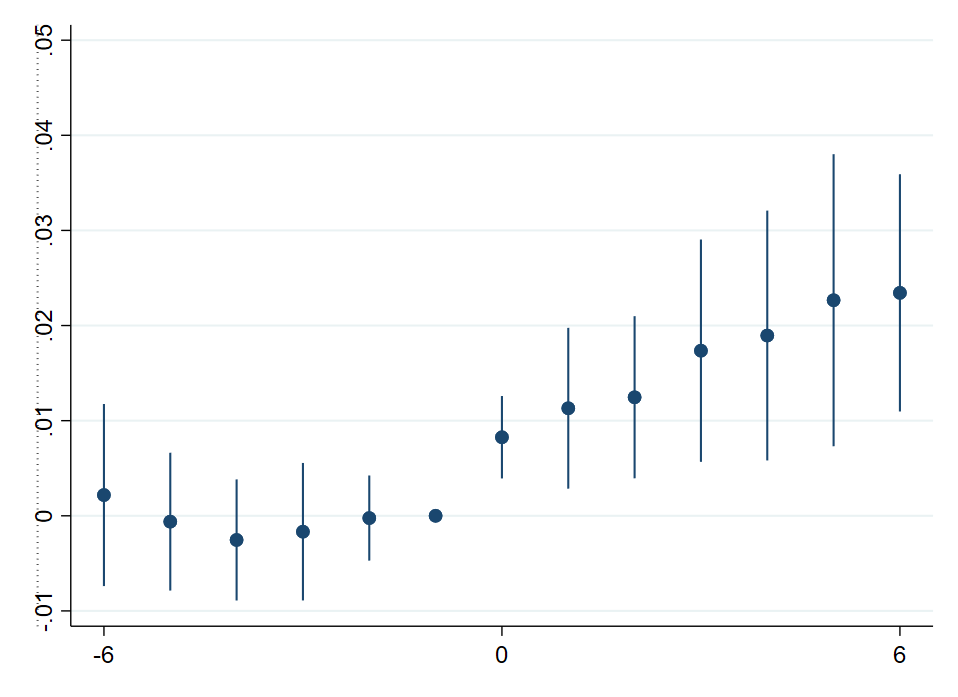
\includegraphics[width=0.95\linewidth]{analysis/event_size_robustness/output/last_rentpsqft_sfcc_event025_w6.png}
        \caption{Selecting events of at least \$0.25} \label{appfig:event_study_025_treated}
    \end{subfigure}%
    \begin{subfigure}{0.5\textwidth} \centering
        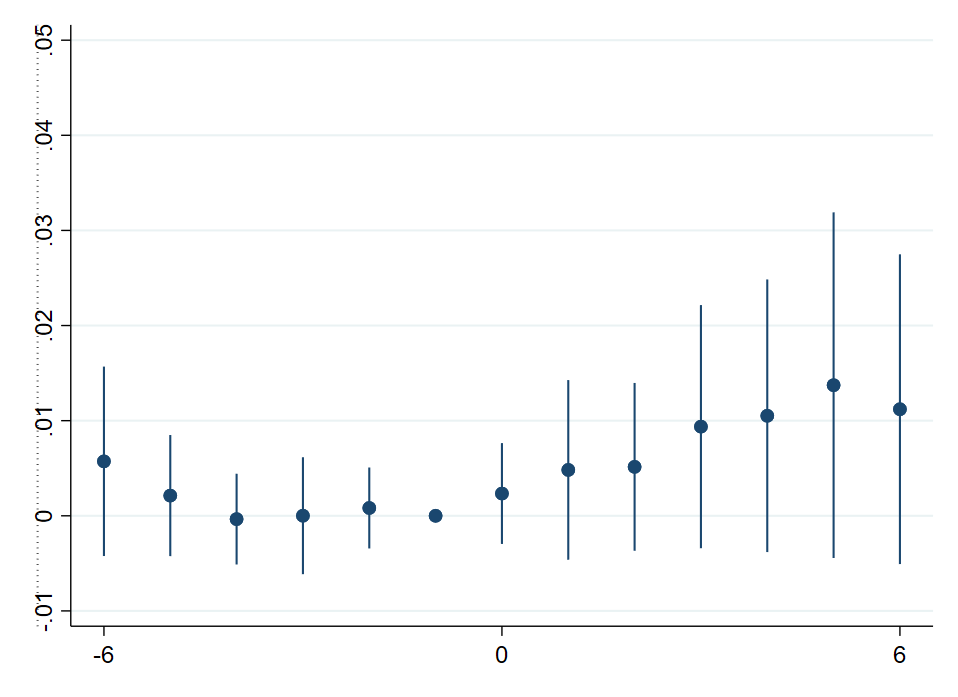
\includegraphics[width=0.95\linewidth]{analysis/event_size_robustness/output/last_rentpsqft_sfcc_event025_w6_county-trend.png}
        \caption{\begin{tabular}{c} Selecting events of at least \$0.25 \\ and county-specific trend \end{tabular}} \label{appfig:event_study_025_treated_county-trends}
    \end{subfigure}\\
    \begin{subfigure}{0.5\textwidth} \centering
        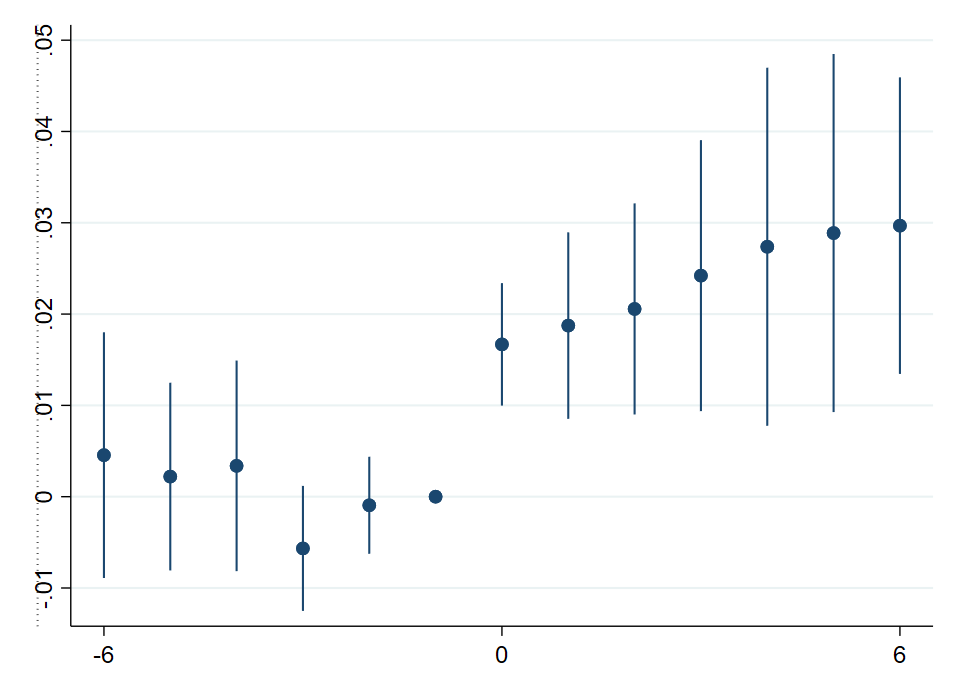
\includegraphics[width=0.95\linewidth]{analysis/event_size_robustness/output/last_rentpsqft_sfcc_event075_w6.png}
        \caption{Selecting events of at least \$0.75} \label{appfig:event_study_025_treated}
    \end{subfigure}%
    \begin{subfigure}{0.5\textwidth} \centering
        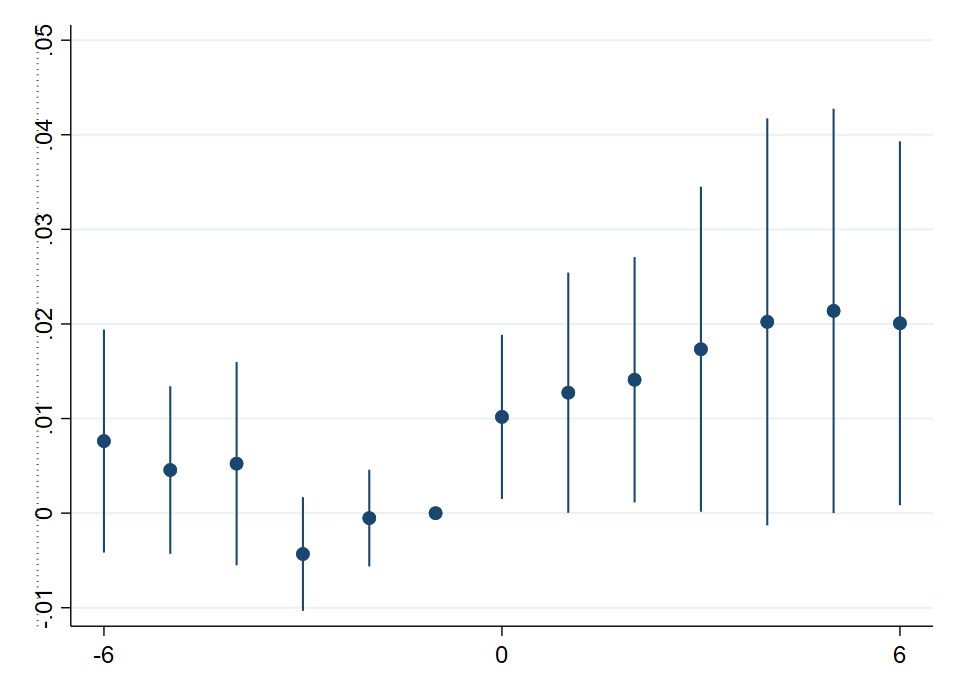
\includegraphics[width=0.95\linewidth]{analysis/event_size_robustness/output/last_rentpsqft_sfcc_event075_w6_county-trend.png}
        \caption{\begin{tabular}{c} Selecting events of at least \$0.75 \\ and county-specific trend \end{tabular}} \label{appfig:event_study_025_treated_county-trends}
    \end{subfigure}\\
    \begin{minipage}{.95\textwidth} \footnotesize
		\vspace{2mm} 
		\textit{Notes}: The figure shows results from fitting the ``last event'' event study with zipcode and calendar time fixed effects, controls for unused events, and including never treated zipcodes (essentially, this is the specification in the bottom row of \ref{fig:event_study_main} without county trends). All of the results select the last minimum wage event per zipcode, based on some cut-off and the requirement that it took place before June 2019 (so that every event has at least 6 months after it). The top row uses a cut-off of \$0.25, whereas the bottom row selects events based on a cut-off of \$0.75. Panels on the right add county-specific trends as controls.
	\end{minipage}
\end{figure}

\clearpage
\begin{figure}[h!] \centering
    \caption{Sensitivity of event study results to rent variable}
    \label{appfig:event_study_change_depvar}
    \begin{subfigure}{0.5\textwidth} \centering
        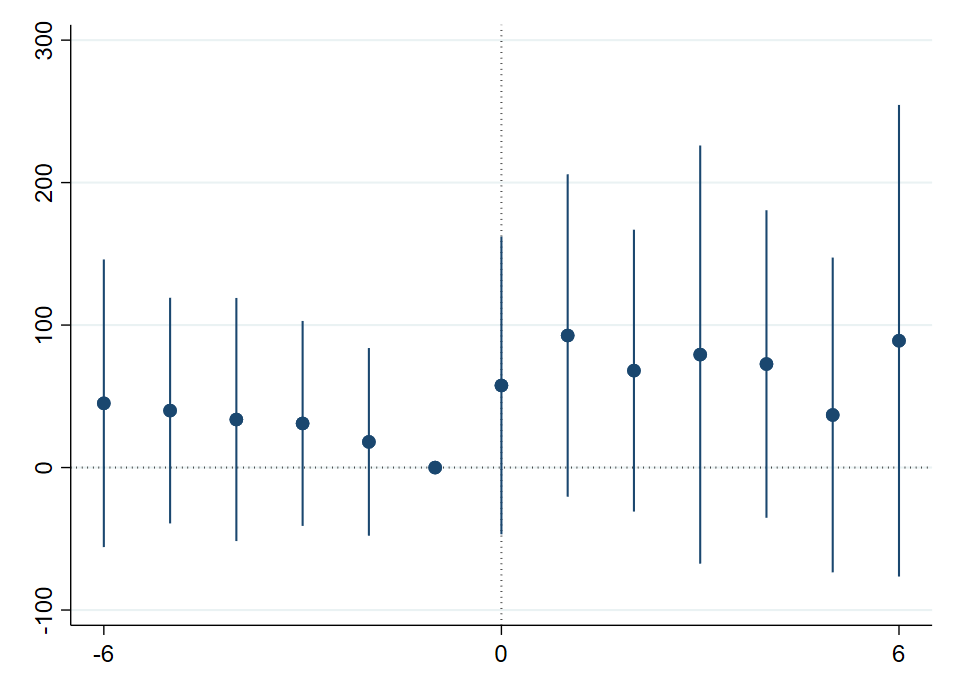
\includegraphics[width=0.95\linewidth]{analysis/event_study/output/last_rent_sfcc_w6.png}
        \caption{SFCC listings} \label{appfig:event_study_SFCC}
    \end{subfigure}%
    \begin{subfigure}{0.5\textwidth} \centering
        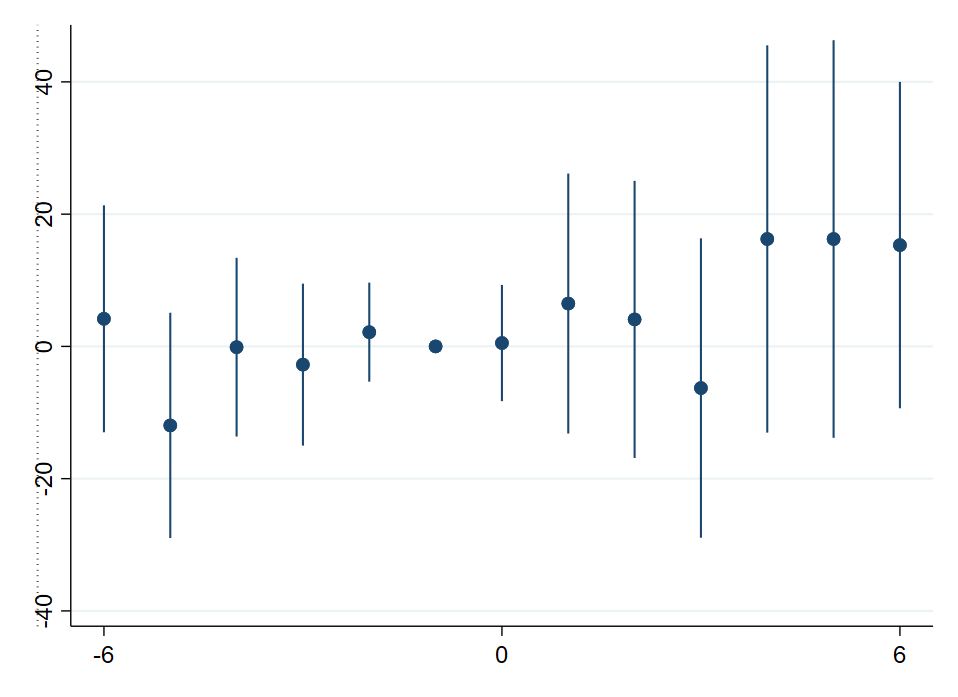
\includegraphics[width=0.95\linewidth]{analysis/event_study/output/last_rent_2br_w6.png}
        \caption{2 bedroom listings} \label{appfig:event_study_2BR}
    \end{subfigure}\\
    \begin{subfigure}{0.5\textwidth} \centering
        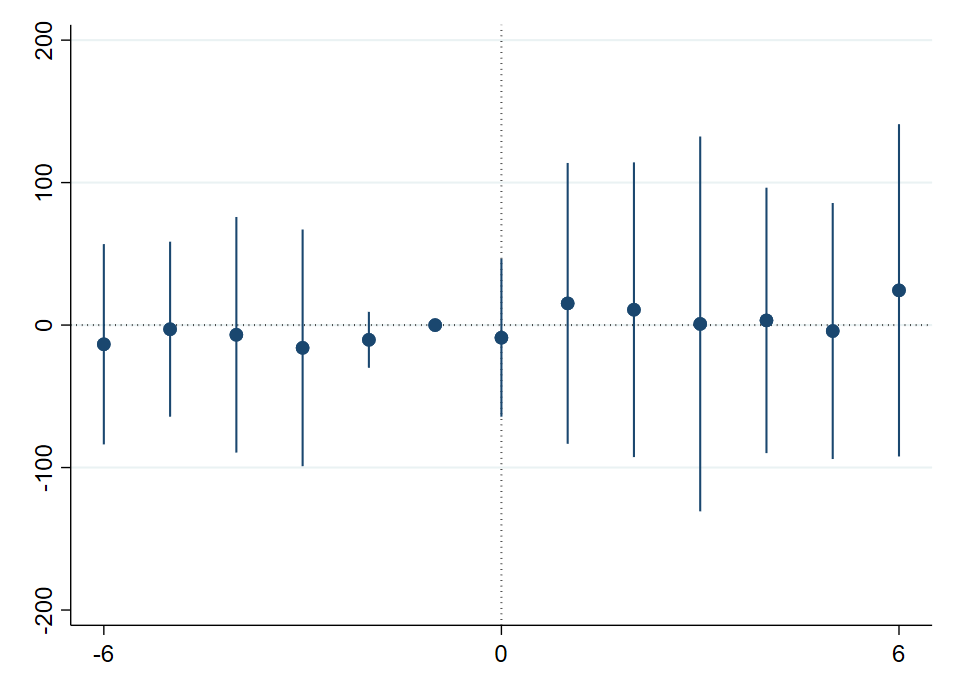
\includegraphics[width=0.95\linewidth]{analysis/event_study/output/last_rent_mfr5plus_w6.png}
        \caption{5 bedroom or more listings} \label{appfig:event_study_5BR}
    \end{subfigure}%
    \begin{subfigure}{0.5\textwidth} \centering
        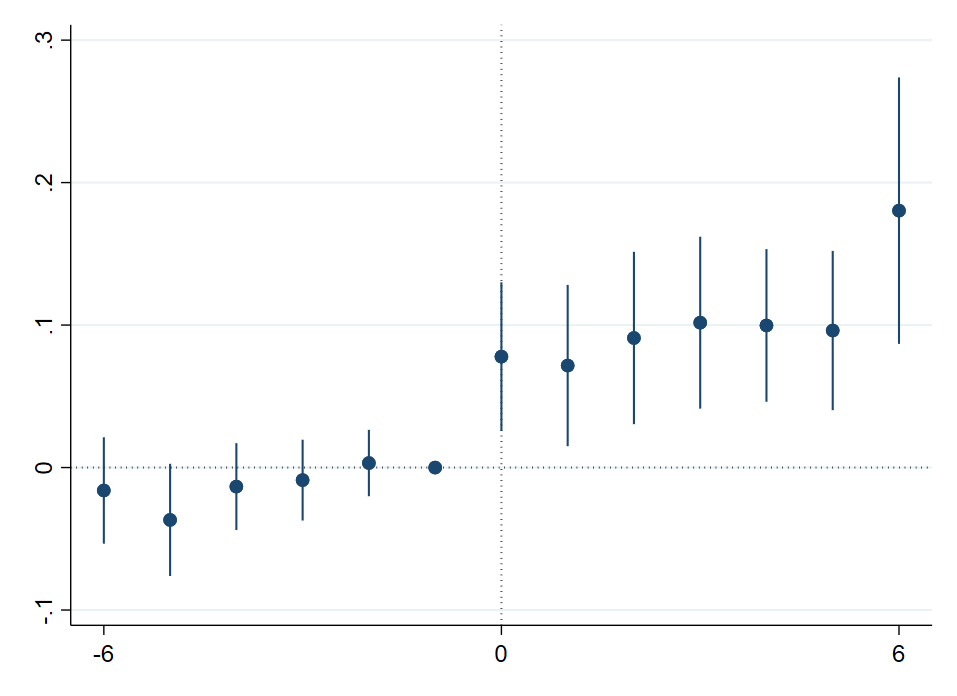
\includegraphics[width=0.95\linewidth]{analysis/event_study/output/last_rentpsqft_sfcc_w6.png}
        \caption{SFCC listings per square foot} \label{appfig:event_study_SFCCpsqft}
    \end{subfigure}\\
    \begin{subfigure}{0.5\textwidth} \centering
        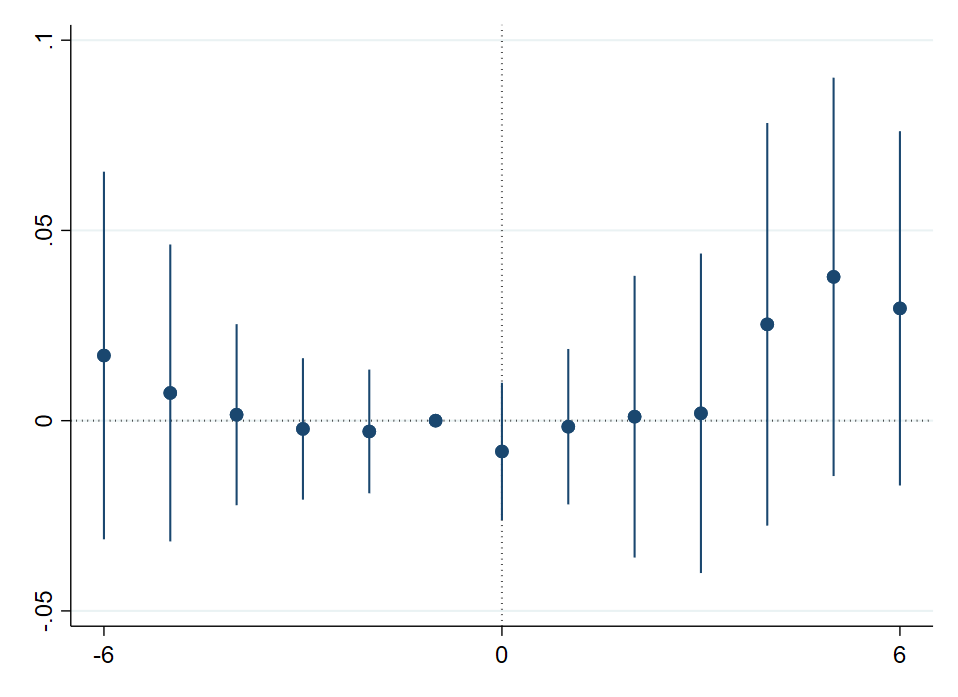
\includegraphics[width=0.95\linewidth]{analysis/event_study/output/last_rentpsqft_2br_w6.png}
        \caption{Two bedroom listings per square foot} \label{appfig:event_study_2BRpsqft}
    \end{subfigure}%
    \begin{subfigure}{0.5\textwidth} \centering
        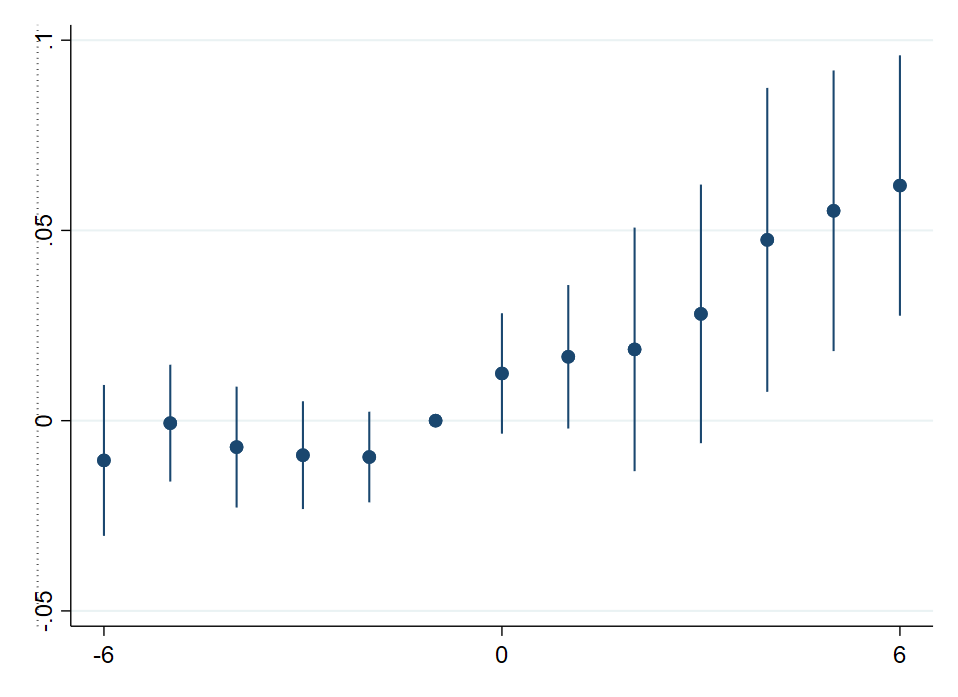
\includegraphics[width=0.95\linewidth]{analysis/event_study/output/last_rentpsqft_mfr5plus_w6.png}
        \caption{5 bedroom or more listings per square foot} \label{appfig:event_study_5BRpsqft}
    \end{subfigure}\\
    \begin{minipage}{.95\textwidth} \footnotesize
		\vspace{2mm} 
		\textit{Notes}: The figure shows results from fitting the ``last event'' event study with zipcode and calendar time fixed effects, controls for unused events, and including never treated zipcodes (essentially, this is the specification in the bottom row of figure \ref{fig:event_study_main} without county trends). All of the results select the last minimum wage event per zipcode under the condition that they were of at least \$0.50. Each panel uses a different variable in the left-hand side of the equation. Panel (a), (b), and (c) use average rents in the categories single family and condos, 2 bedroom, and 5 bedroom or more, respectively. Importantly, these do not control for size of the listing. Panels (d), (e), and (f) show results for the same three variables per square foot. Note that panel (d) in this figure is the same as panel (e) in figure \ref{fig:event_study_main}. The number of observations in each regression are: (a) $N = 125,644$, (b) $N = 32,426$, (c) $N = 47,090$, (d) $N = 113,375$, (e) $N = 24,782$, (f) $N = 37,588$.
	\end{minipage}
\end{figure}


\clearpage
\begin{figure}[htb] \centering
    \caption{Heterogeneity of effect - first difference model}
    \label{appfig:fd_heterogeneity_appendix}
    \begin{subfigure}{0.5\textwidth} \centering
        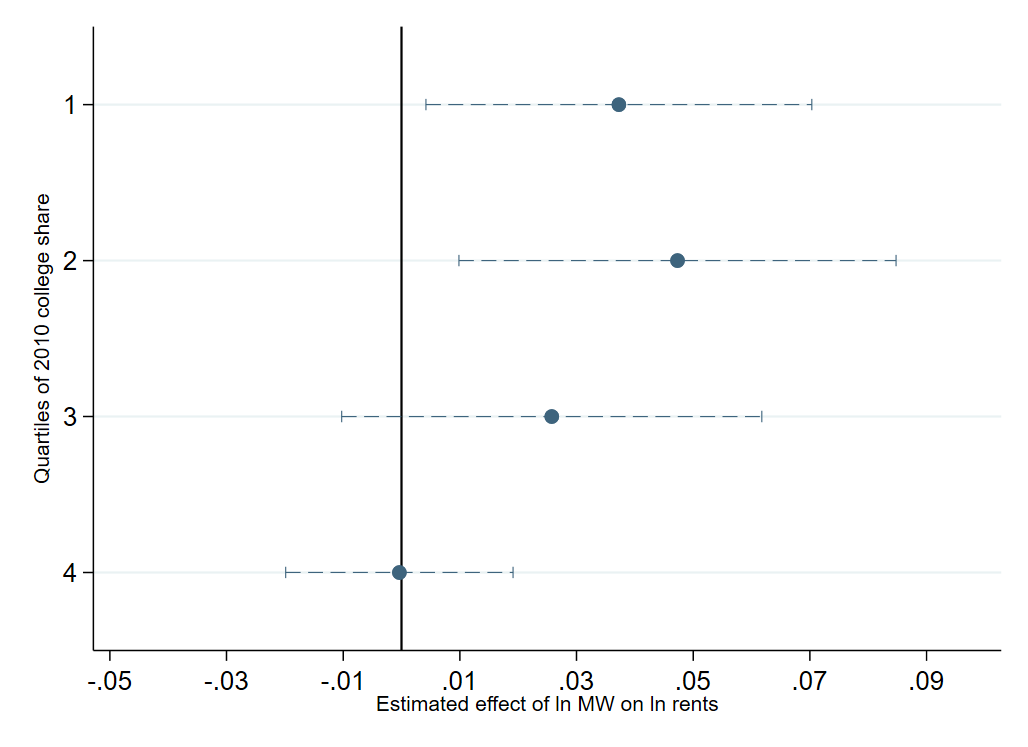
\includegraphics[width=0.99\linewidth]{analysis/first_differences/output/fd_static_heter_college_share20105.png}
        \caption{Share of college graduates in zipcode} \label{appfig:fd_heterogeneity_college_share}
    \end{subfigure}%
    \begin{subfigure}{0.5\textwidth} \centering
        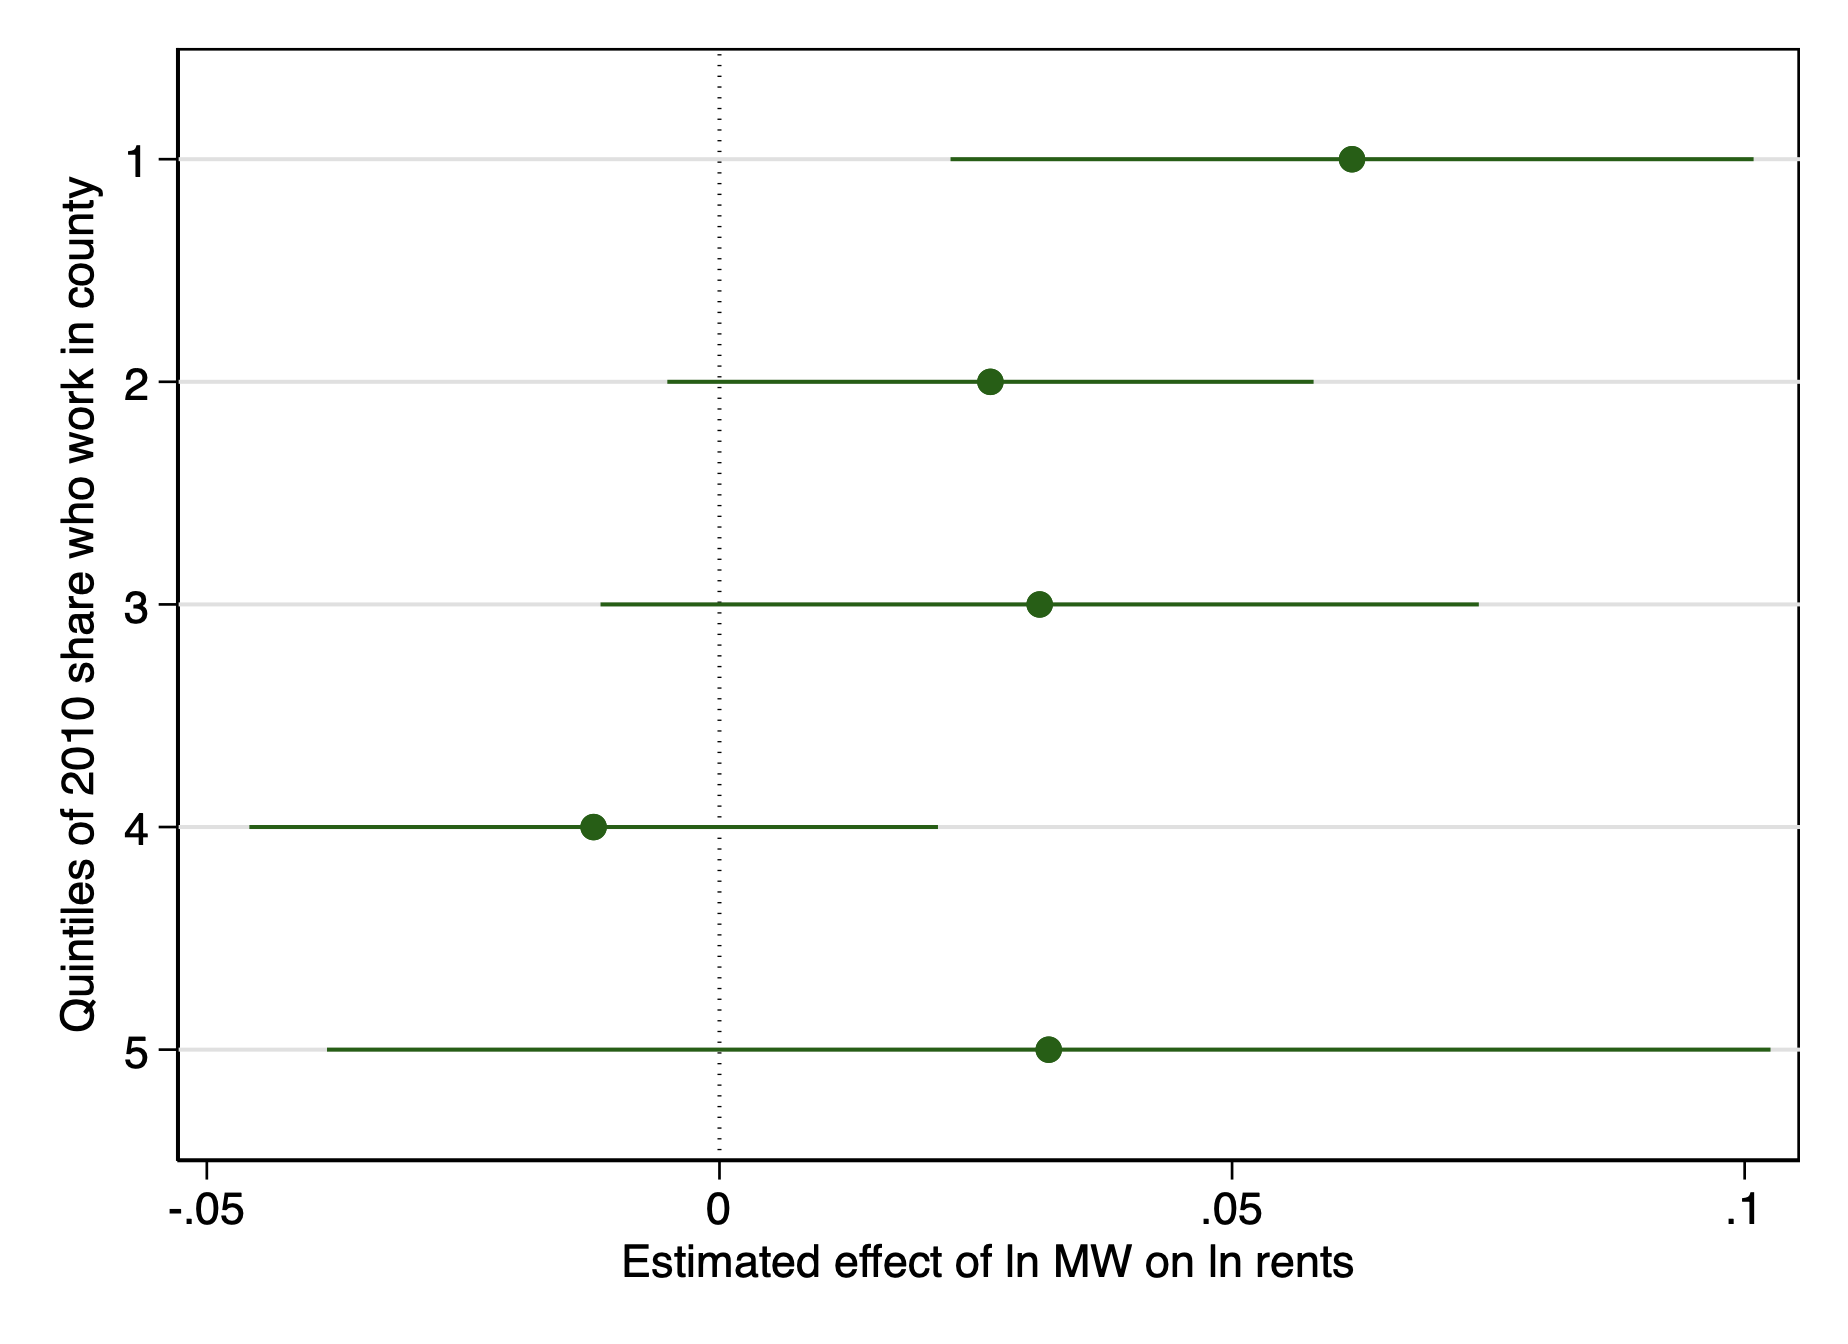
\includegraphics[width=0.99\linewidth]{analysis/first_differences/output/fd_static_heter_work_county_share20105.png}
        \caption{Share of individuals in zipcode who work in county} \label{appfig:fd_heterogeneity_work_county}
    \end{subfigure}\\
    \begin{subfigure}{0.5\textwidth} \centering
        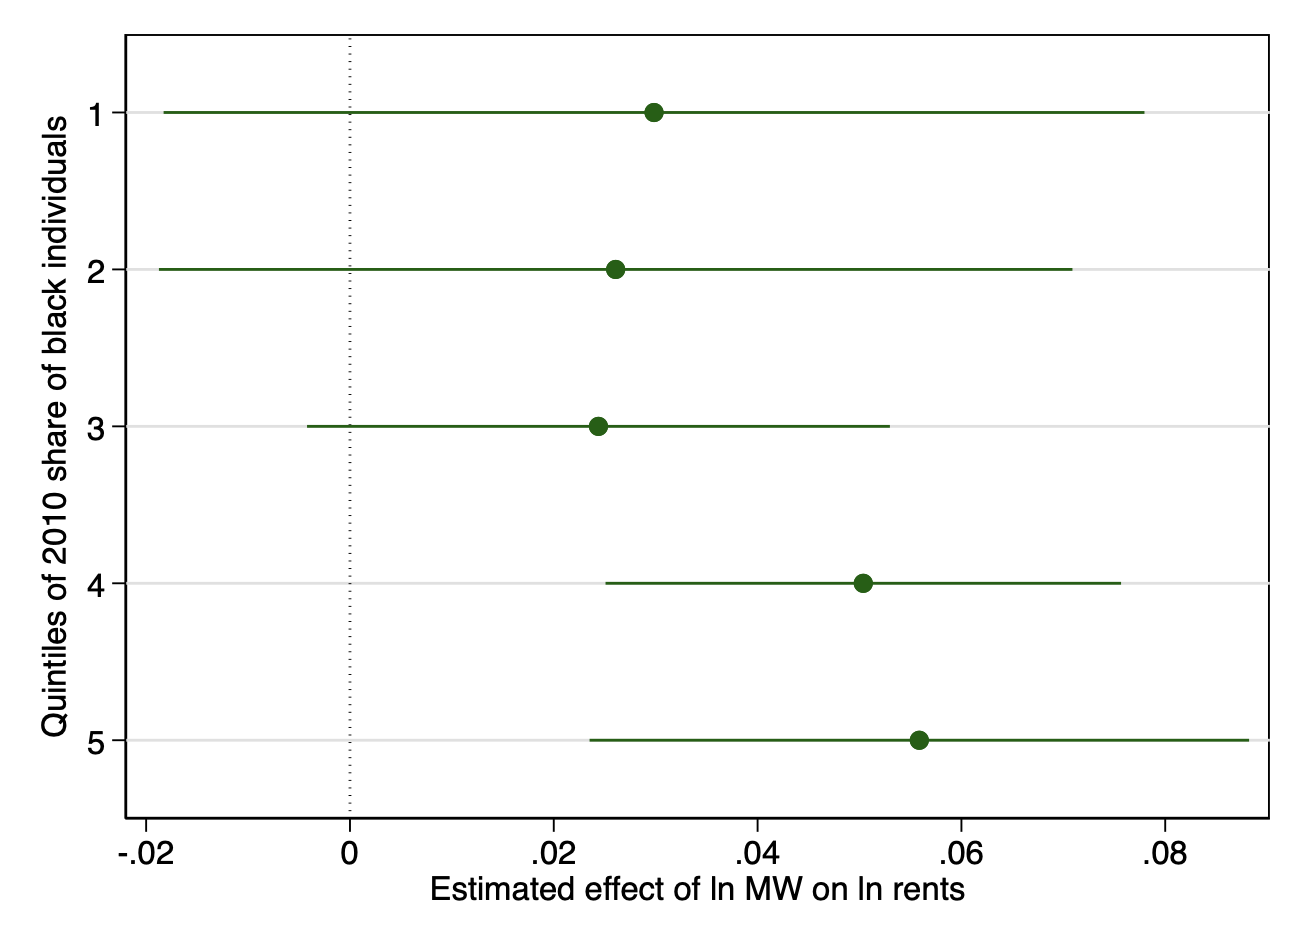
\includegraphics[width=0.99\linewidth]{analysis/first_differences/output/fd_static_heter_black_share2010.png}
        \caption{Share of black individuals} \label{appfig:fd_heterogeneity_work_county}
    \end{subfigure}\\
    \begin{minipage}{.95\textwidth} \footnotesize
		\vspace{2mm} 
		\textit{Notes}: The figure shows 
	\end{minipage}
\end{figure}

